\documentclass[12pt]{article}

\usepackage{setspace}
\usepackage{caption}
\usepackage{subcaption}
\usepackage{float}
\usepackage{amsmath}
\usepackage{graphicx}
\graphicspath{ {./images/} }
\usepackage[utf8]{inputenc}
\usepackage[russian]{babel}

\usepackage{geometry}
 \geometry{
 a4paper,
 left=20mm,
 right=20mm,
 top=20mm,
 bot=20mm,
 }

\begin{document}

\begin{titlepage}
\begin{center}
    {\small НАЦИОНАЛЬНЫЙ ИССЛЕДОВАТЕЛЬСКИЙ УНИВЕРСИТЕТ ИТМО} \\
    {\small Факультет систем управления и робототехники} \\
    \vspace*{10\baselineskip}
    {\LARGEЭлектроника и схемотехника} \\
    \ \\
    \begin{spacing}{1.5}
    {\large Лабораторная работа №2 \\
    Исследование характеристик биполярного транзистора и расчёт усилительного каскада} \\
    \end{spacing} \\
    \ \\
    Вариант 2 \\
    \vspace*{10\baselineskip}
    \hfill {Выполнили студенты:} \\
    \hfill {Кирбаба Д.Д. R3338} \\
    \hfill {Курчавый В.В. R3338} \\
    \ \\
    \hfill {Преподаватель:} \\
    \hfill {Николаев Н.А.} \\
    \mbox{}
    \vfill {г. Санкт-Петербург\\2023}
\end{center}
\end{titlepage}

\section*{Цель работы}
\begin{itemize}
  \item Получение входной характеристики и семейства выходных характеристик биполярного транзистора в схеме с общим эмиттером;
  \item Расчёт усилительного каскада с заданием рабочей точки транзистора с помощью отрицательной обратной связи по току.
\end{itemize}

\section*{Ход работы}
Вариант 2: транзистор 2N2369, $E_C = 15 \ V$.

\begin{figure}[H]
    \centering
    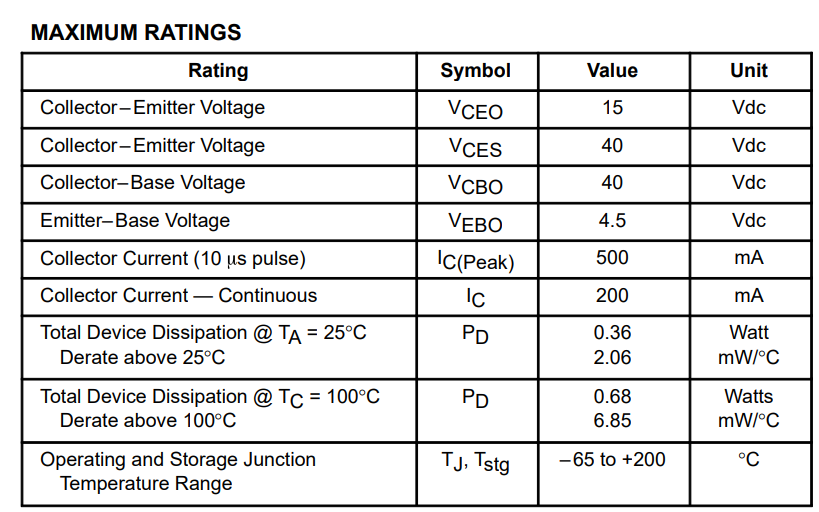
\includegraphics[width=0.7\textwidth]{transistor_datasheet_1.png}
    \caption{Характеристики транзистора 1.}
    \label{fig:transistor_datasheet_1.png}
\end{figure}
\begin{figure}[H]
    \centering
    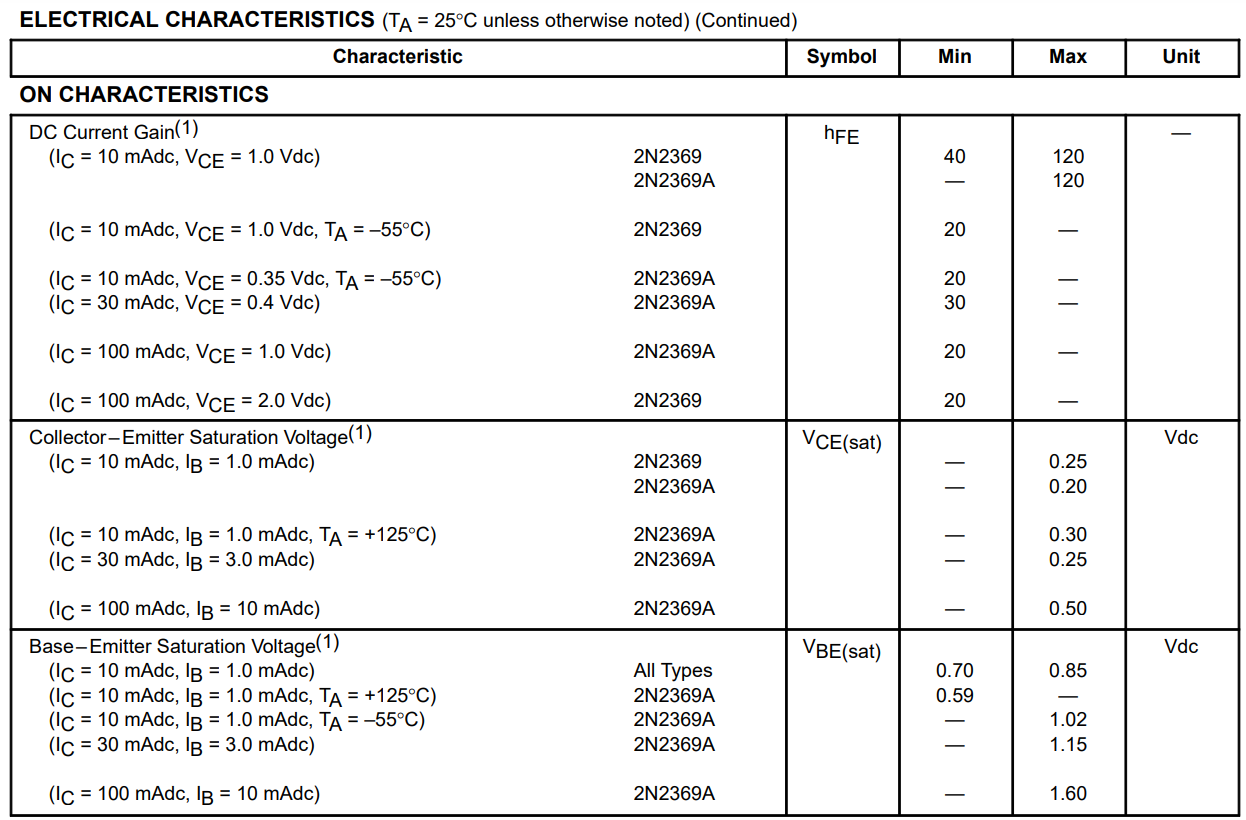
\includegraphics[width=0.7\textwidth]{transistor_datasheet_2.png}
    \caption{Характеристики транзистора 2.}
    \label{fig:transistor_datasheet_2.png}
\end{figure}
\ \\
Максимальный ток коллектора: $I_{C_{peak}} = 0.2 \ A$.\\
Максимальное напряжение коллектор-эмиттер: $U_{CEO} = 15 \ V$.\\
Коэффициент усиления по току: $h_{FE} = [40; \ 120]$. \\
Максимальная рассеиваемая мощность: $P_D = 0.36 \ W$.\\

\subsubsection*{Получение входной характеристики биполярного транзистора}
Построим входную харатеристику транзистора (шаг напряжения $0.001 \ V$).
\begin{figure}[H]
    \centering
    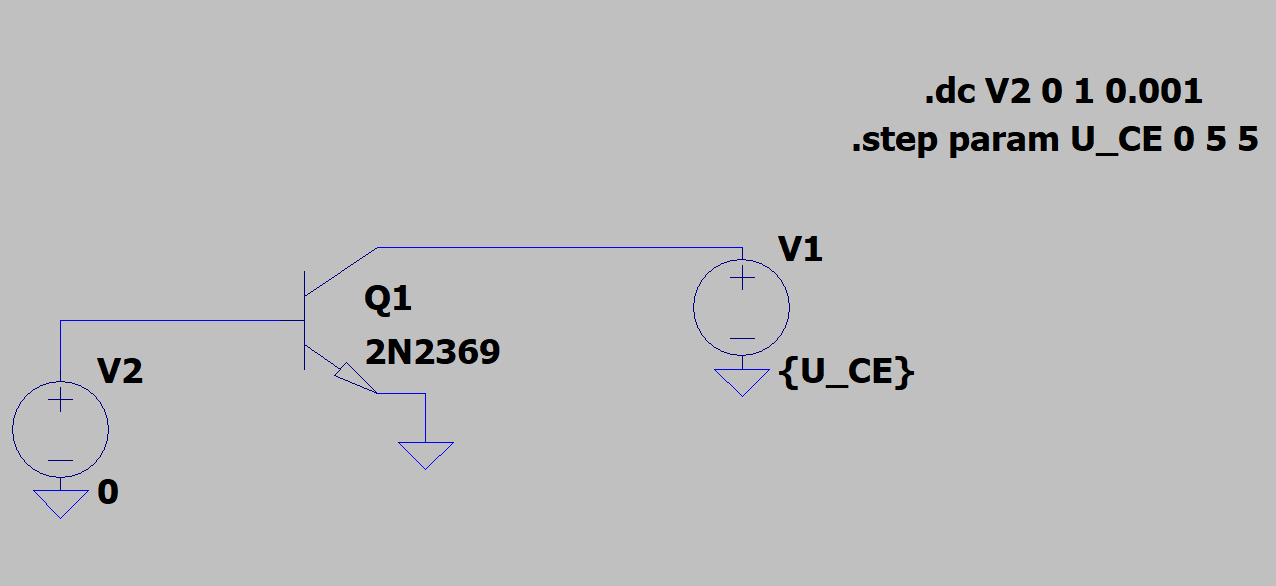
\includegraphics[width=0.7\textwidth]{1_scheme.png}
    \caption{Схема для моделирования входной характеристики транзистора.}
    \label{fig:1_scheme.png}
\end{figure}\\

\begin{figure}[H]
    \centering
    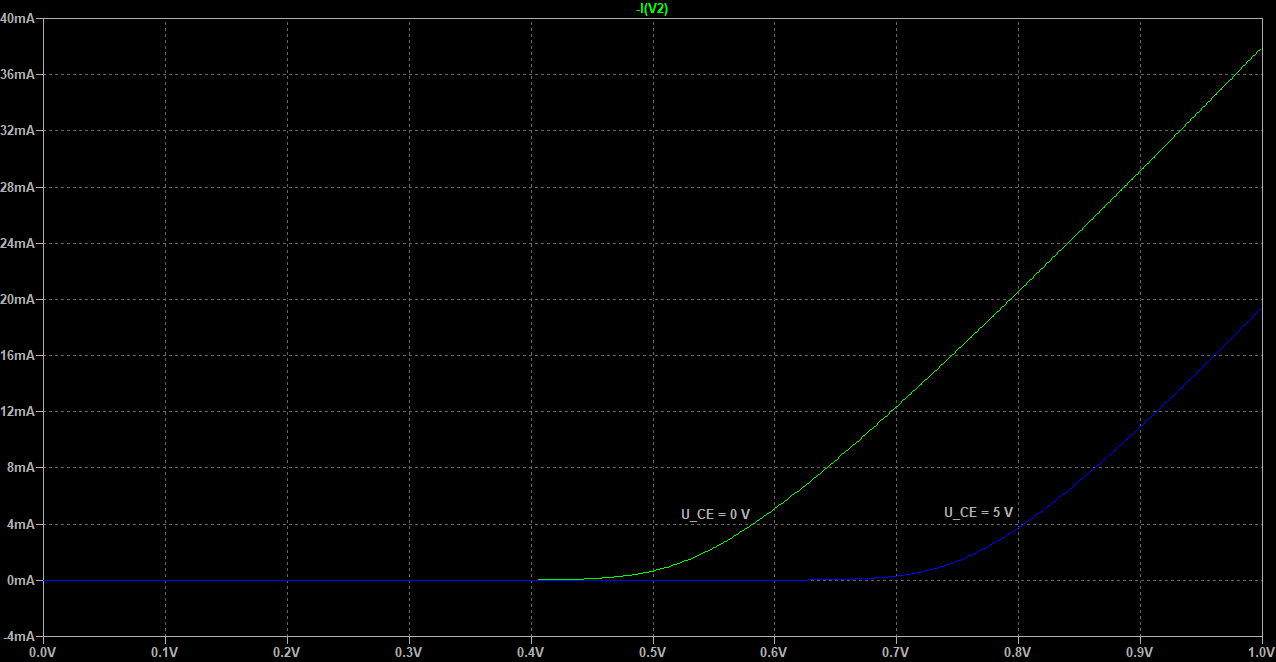
\includegraphics[width=\textwidth]{1_input_char.png}
    \caption{Входная характеристика.}
    \label{fig:1_input_char.png}
\end{figure}\\
Рассчитаем дифференциальное входное сопротивление транзистора:
\[
r_{in} = \frac{\delta U_{BE}}{\delta I_B} = \frac{984.67 - 859.8}{18.096 - 7.805} = 12.134 \ \text{Ohm}
\]

\subsubsection*{Получение семейства выходных характеристик биполярного транзистора}
\begin{figure}[H]
    \centering
    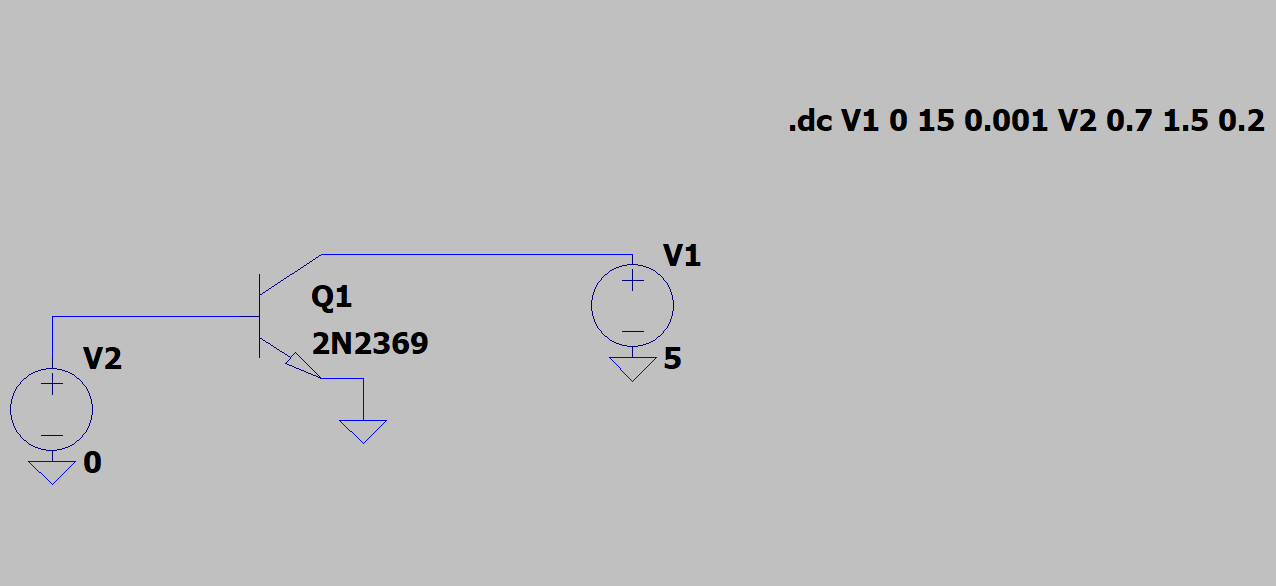
\includegraphics[width=0.7\textwidth]{2_scheme.png}
    \caption{Схема для получения семейства выходных характеристик транзистора.}
    \label{fig:2_scheme.png}
\end{figure}
\begin{figure}[H]
    \centering
    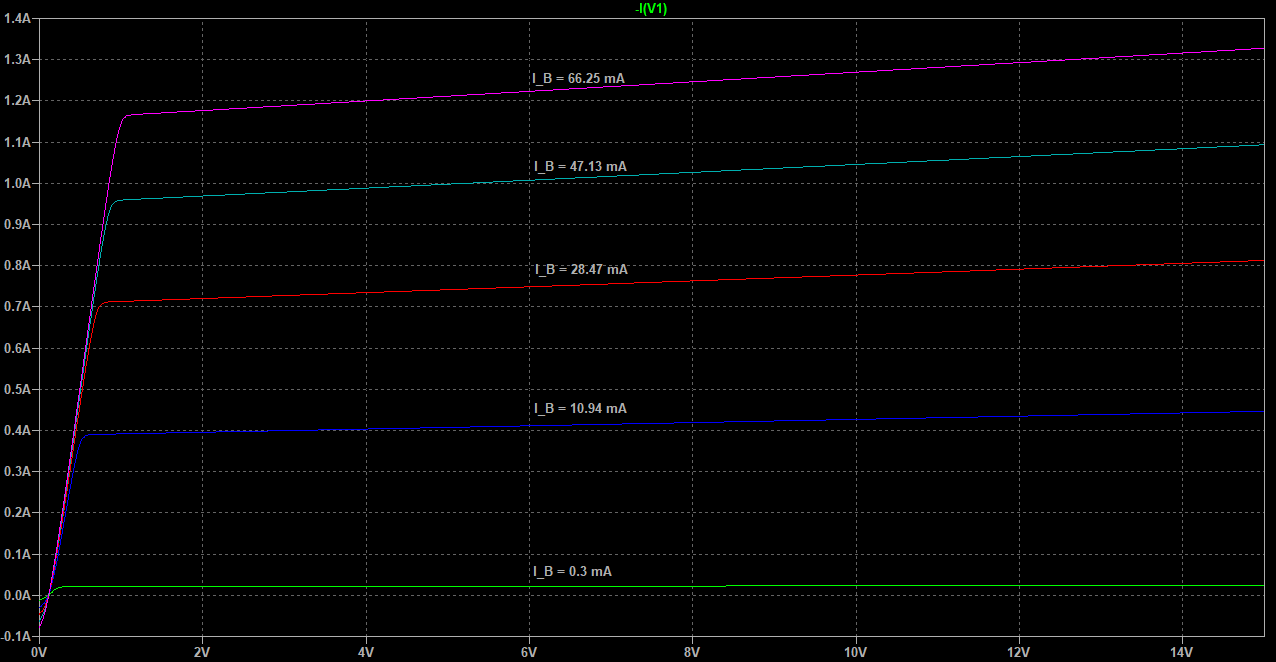
\includegraphics[width=\textwidth]{2_output_char.png}
    \caption{Семейство выходных характеристик.}
    \label{fig:2_output_char.png}
\end{figure}
Определим для каждой полученной выходной характеристики значение тока коллектора, соответствующее напряжению коллектор-эмиттер $U_{KE} = 5 \ V$ (нумерация выходных характеристик сверху-вниз):
\begin{align*} 
I_{C1} = 0.02186 \ A \\ 
I_{C2} = 0.4074 \ A \\
I_{C3} = 0.7417 \ A \\
I_{C4} = 0.9978 \ A \\
I_{C5} = 1.2114 \ A
\end{align*}
Рассчитаем коэффициент передачи тока:
\[
\beta_{AC} = \frac{\delta I_C}{\delta I_B} = \frac{1.2114 - 0.02186}{0.06625 - 0.0003} = 18.037
\]

\subsubsection*{Задание рабочей точки с помощью отрицательной обратной связи по току}
Определим рабочий диапазон транзистора, зная что его ограничения:
\[
I_{C_{peak}} = 0.2 \ A, \ 
U_{CEO} = 15 \ V, \ 
P_D = 0.36 \ W.
\]
\begin{figure}[H]
    \centering
    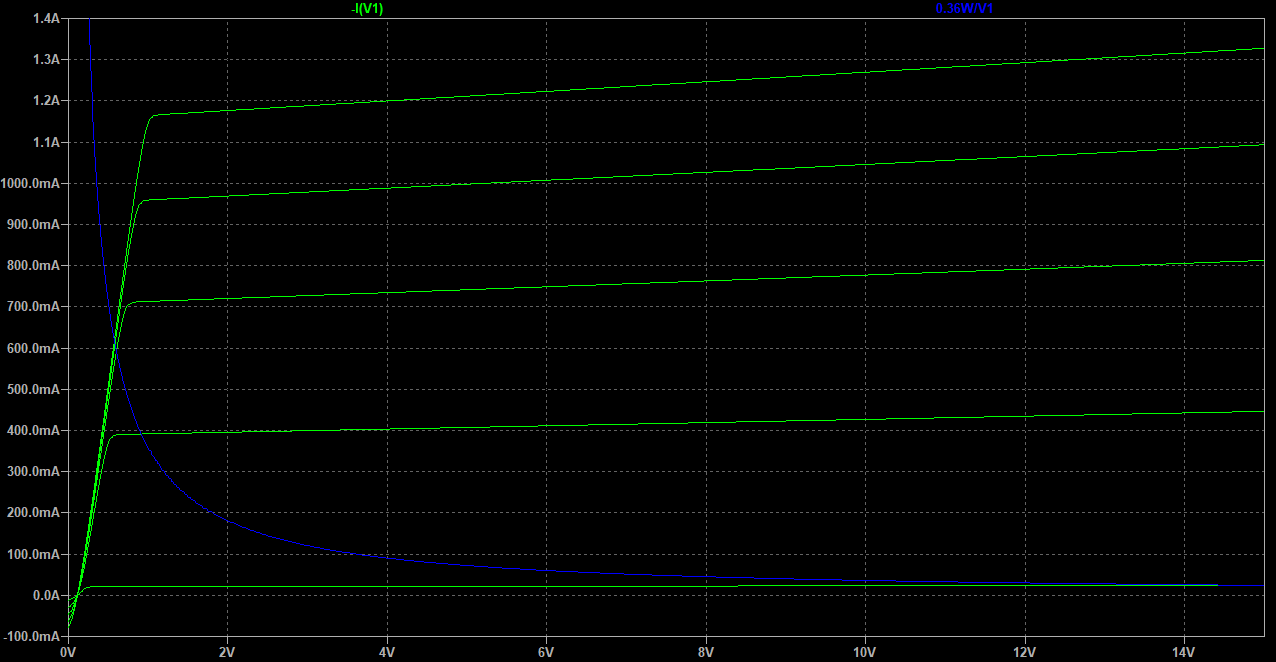
\includegraphics[width=\textwidth]{3_output_char_w_max_p_line.png}
    \caption{Линия максимальной мощности на семействе ВАХ.}
    \label{fig:3_output_char_w_max_p_line.png}
\end{figure}
\ \\
Рабочий диапазон транзистора будет находиться под данной линией мощности, а также ограничен прямыми $I = I_{C_{peak}} = 0.2 \ A, \ U = U_{CEO} = 15 \ V.$ \\
\ \\
Так как пиковое значение коллектора $0.2 \ A$, а почти все построенные выходные характеристики соответствуют большему значению, то построим семейство с меньшими силами тока на базе, а следовательно с меньшими силами тока на коллекторе:
\begin{figure}[H]
    \centering
    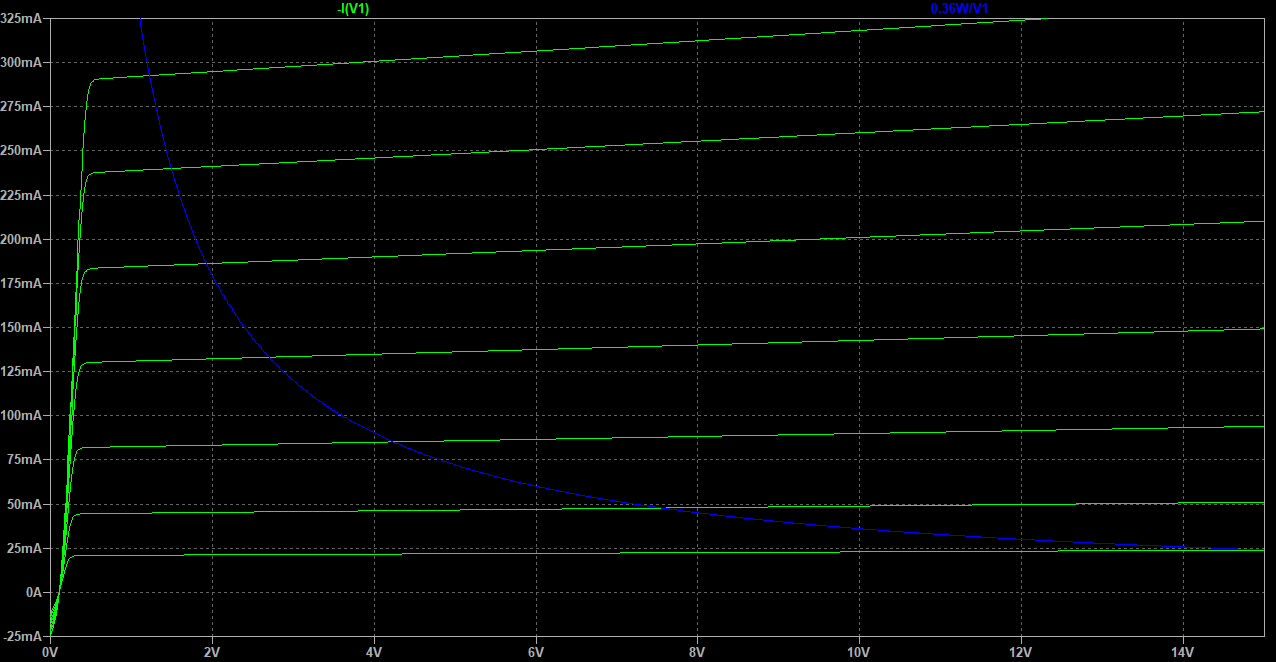
\includegraphics[width=\textwidth]{3_small_output_char_w_max_p_line.png}
    \caption{Семейство ВАХ с меньшими силами тока на базе.}
    \label{fig:3_small_output_char_w_max_p_line.png}
\end{figure}
Построим нагрузочную линию (учитывая что $E_k = 15 \ V$). Она должна проходить через $(E_k, \ 0).$ И выберем рабочую точку.
\begin{figure}[H]
    \centering
    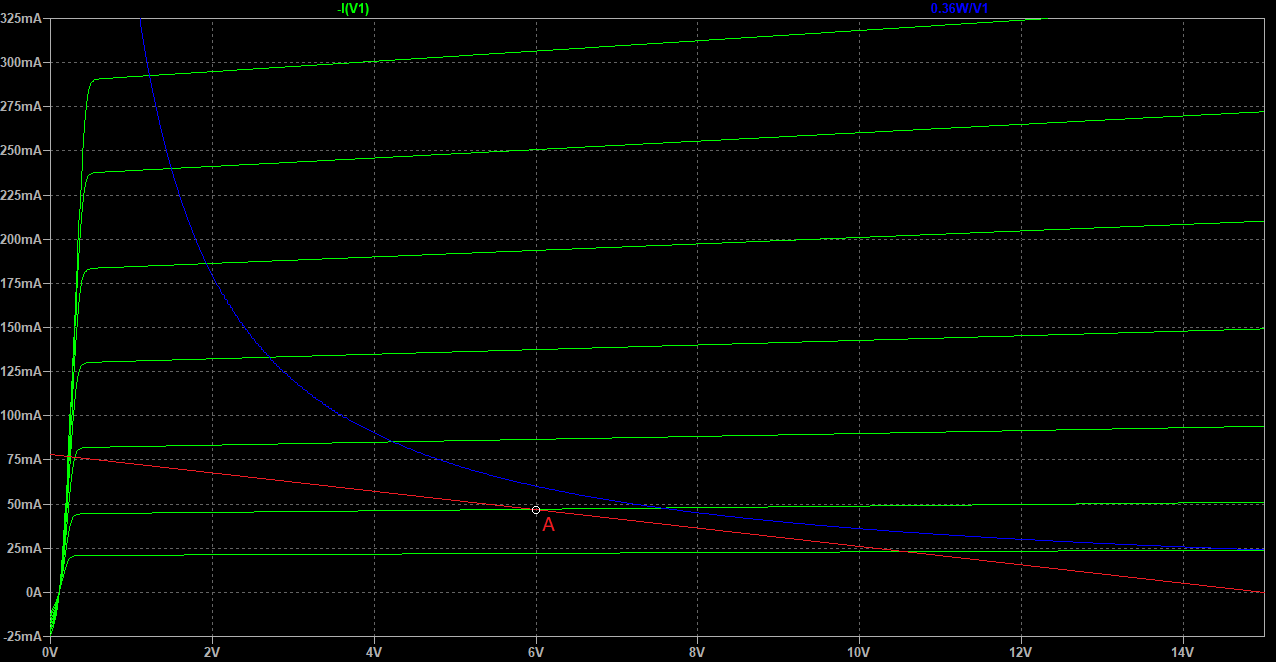
\includegraphics[width=\textwidth]{3_small_output_char_w_max_p_load_lines_and_A.png}
    \caption{Нагрузочная прямая и рабочая точка на семействе ВАХ.}
    \label{fig:3_small_output_char_w_max_p_load_lines_and_A.png}
\end{figure}

Координаты точки $A = (6 \ V, \ 47.062 \ mA)$.\\
Точка лежит на линии выходной характеристики с $I_{B_A} = 690 \ \mu A$.

\begin{figure}[H]
    \centering
    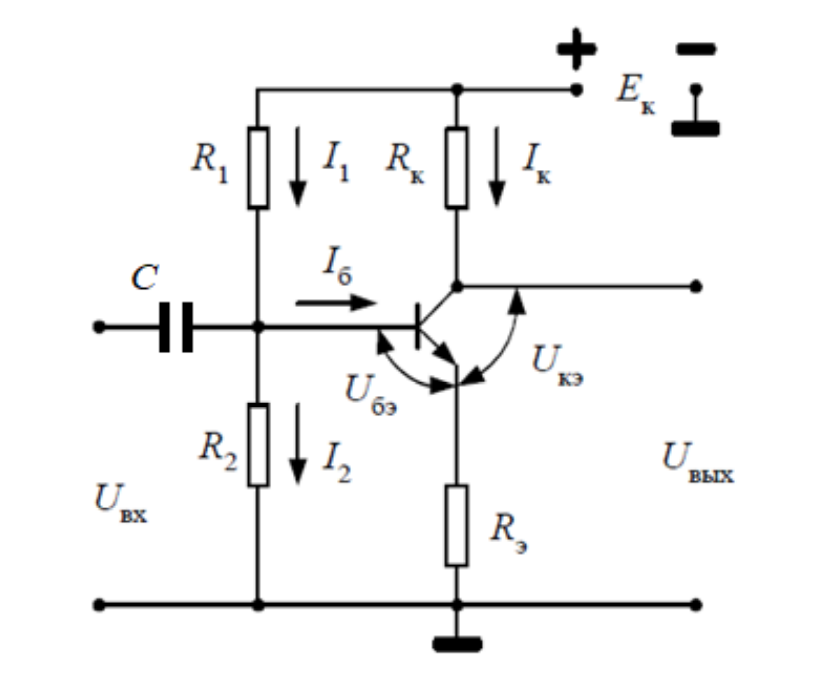
\includegraphics[width=0.5\textwidth]{3_scheme_book.png}
    \caption{Схема с ООС по току.}
    \label{fig:3_scheme_book.png}
\end{figure}

Для расчета транзистора по постоянному току необходимо определить номинальные значения резисторов, которые задают рабочую точку транзистора. \\
Резисторы служат для задания рабочей точки, конденсатор большой емкости (примерно 1 мкФ) выполняет роль гальванической развязки по постоянному току. В данном случае необходимо найти величины  сопротивлений $R_C, \ R_1, \ R_2, \ R_E.$ \\
По нагрузочной прямой найдем максимальное значение тока насыщения транзистора $I_{CS}$ - это ток в точке пересечения нагрузочной прямой и оси тока, то есть 
\[
I_{CS} = 78 \ mA
\]
Величина сопротивления резистора в цепи коллектора:
\[
R_C = \frac{E_C}{I_{CS}} = 192.30 \ Ohm = |E192| = 193 \ Ohm
\]
По величине тока базы в точке А, определим падение напряжения на базе:

\begin{figure}[H]
    \centering
    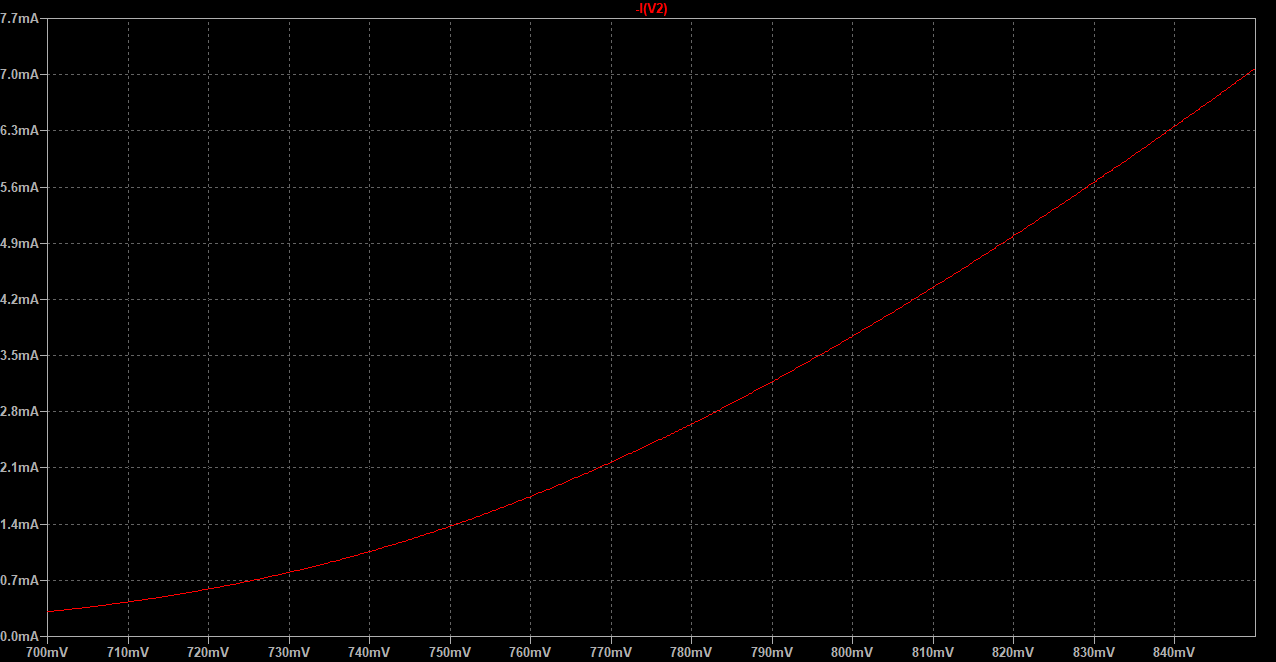
\includegraphics[width=\textwidth]{3_input_char.png}
    \caption{Входная характеристика.}
    \label{fig:3_input_char.png}
\end{figure}

\[
U_{BE_A} = 725.1 \ mV
\]
Ток эмиттера является суммой токов коллектора и базы:
\[
I_{E_A} = I_{B_A} + I_{C_A} = 0.047752 \ A
\]
Уравнение равновесия напряжений по второму закону Кирхгофа для цепи эмиттер-коллектор имеет вид:
\[
E_C = I_{C_A} R_C + U_{CE} + I_{E_A} * R_E
\]
Для входной цепи по второму закону Кирхгофа можно составить два уравнения равновесия напряжений:
\[
E_C = I_1 R_1 + I_2 R_2
\]
\[
E_C = I_1 R_1 + U_{BE_A} + U_{R_E} = I_1 R_1 + U_{BE_A} + I_{E_A} R_E
\]
Следовательно:
\[
U_{R_2} = I_2 R_2 = U_{R_E} + U_{BE_A} = I_{E_A} R_E + U_{BE_A}
\]
Сопротивление $R_E$ осуществляет отрицательную обратную связь по току. Падение напряжения на нём должно быть небольшим, поэтому обычно из практических соображений выбирают:
\[
U_{R_E} = (0.1 / 0.3) E_C
\]
Учитывая это соотношение, можно найти значение сопротивления в цепи эмиттера:
\[
    R_E = \frac{U_{R_E}}{I_{E_A}} = \frac{(0.1/0.3)E_C}{I_{E_A}} = 104.708 \ Ohm = |E192| = 105 \ Ohm 
\]
Падение напряжения на эмиттерном сопротивлении будет равно:
\[
U_{R_E} = I_{E_A} * R_E = 5.01396 \ V
\]
Теперь $U_{R_2}$ может быть рассчитано:
\[
U_{R_2} = U_{R_E} + U_{BE_A} = 5.73906 \ V
\]
Для расчета сопротивления $R_2$ необходимо знать величину тока $I_2$. Из практических соображений значение тока $I_1$ равно:
\[
I_1 = 5 I_{B_A} = 3.45 \ mA
\]
Тогда:
\[
I_2 = I_1 - I_{B_A} = 2.76 \ mA
\]
Теперь можно рассчитать величину сопротивления резистора $R_2$:
\[
R_2 = \frac{U_{R_2}}{I_2} = 2079.34 \ Ohm = |E192| = 2080 \ Ohm
\]
И величина сопротивления резистора $R_1$:
\[
R_1 = \frac{E_C - U_{R_2}}{I_1} = 2684.33 \ Ohm = |E192| = 2670 \ Ohm
\]

\begin{figure}[H]
    \centering
    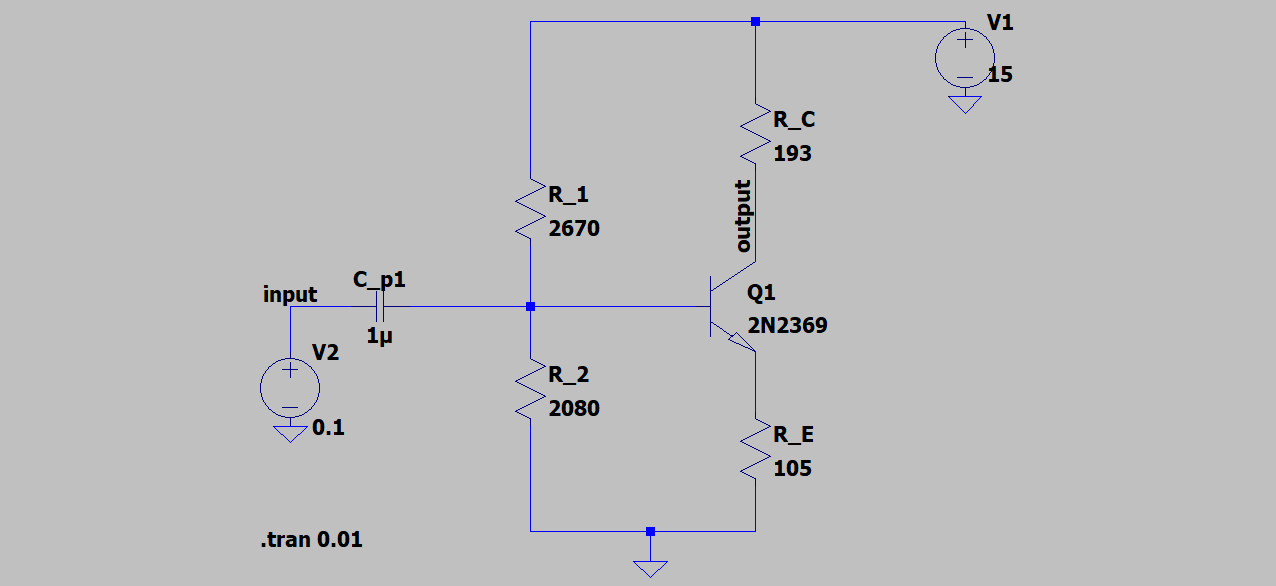
\includegraphics[width=\textwidth]{3_scheme.png}
    \caption{Схема усилителя с биполярным транзистором.}
    \label{fig:3_scheme.png}
\end{figure}

Произведем моделирование работы схемы при постоянном входном сигнале $U_in = 0.1 \ V.$
\begin{figure}[H]
    \centering
    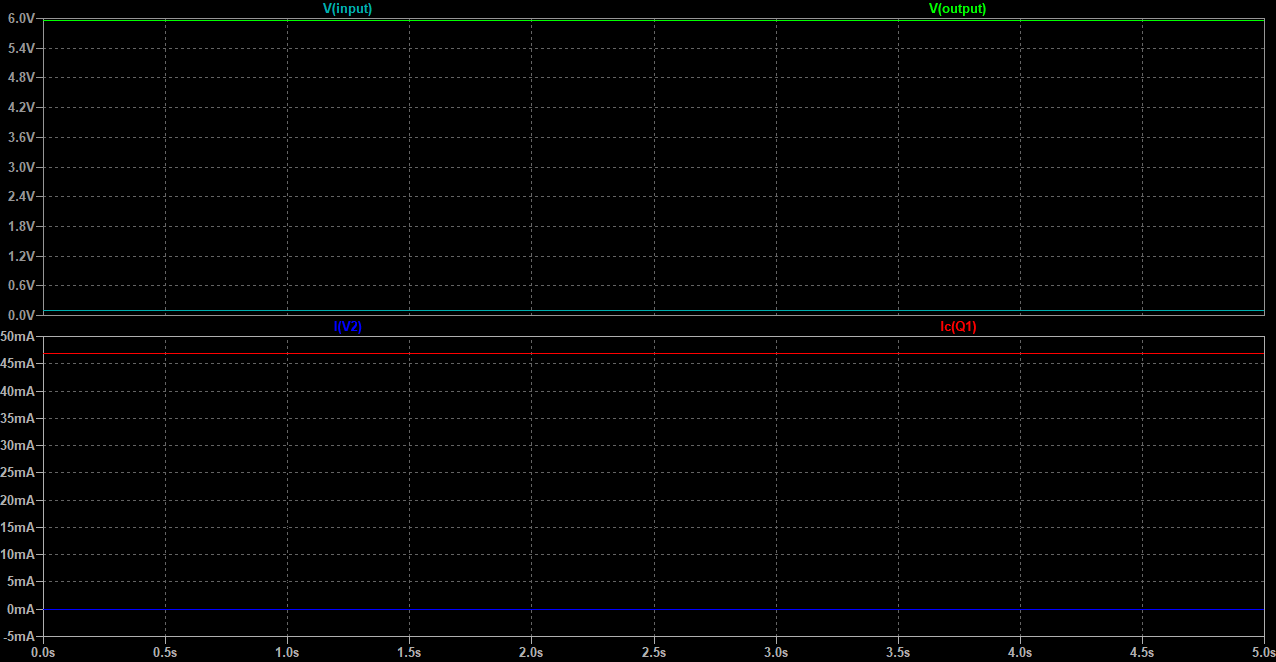
\includegraphics[width=\textwidth]{3_const_i_v.png}
    \caption{Осциллограммы входных и выходных тока и напряжения при постоянном сигнале.}
    \label{fig:3_const_i_v.png}
\end{figure}

Выбранная рабочая точка была $A = (6 \ V, \ 47.062 \ mA)$, выходные ток и напряжение достаточно близки к данным значениям, а именно $I_{out} = 46.866 \ mA, \ U_{out} =  5.955 \ V.$ \\
\ \\
Произведем теперь моделирование работы схемы при гармоническом входном сигнале $0.1 \sin{1000 U}$:
\begin{figure}[H]
    \centering
    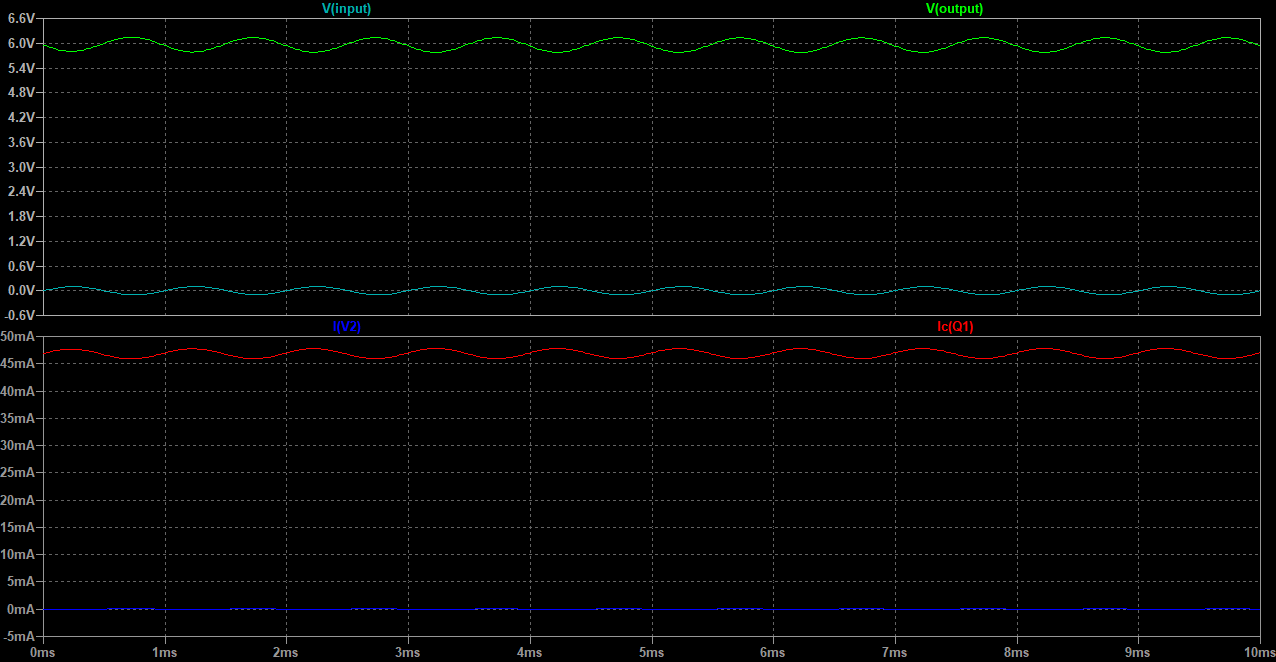
\includegraphics[width=\textwidth]{3_sin_i_v.png}
    \caption{Осциллограммы входных и выходных тока и напряжения при гармоническом сигнале.}
    \label{fig:3_sin_i_v.png}
\end{figure}
Опять убеждаемся, что выходные характеристики соответсвуют заданной рабочей точке.\\
\ \\
Рассчитаем коэффициенты усиления по напряжению и току:
\[
k_I = \frac{46.866 \cdot 10^{-3}}{723 \cdot 10^{-6}} = 64.822
\]
Данное значение попадает в интервал, данный производителем.
\[
k_U = \frac{5.955}{0.1} = 59.55
\]
Проведем частотный анализ схемы:
\begin{figure}[H]
    \centering
    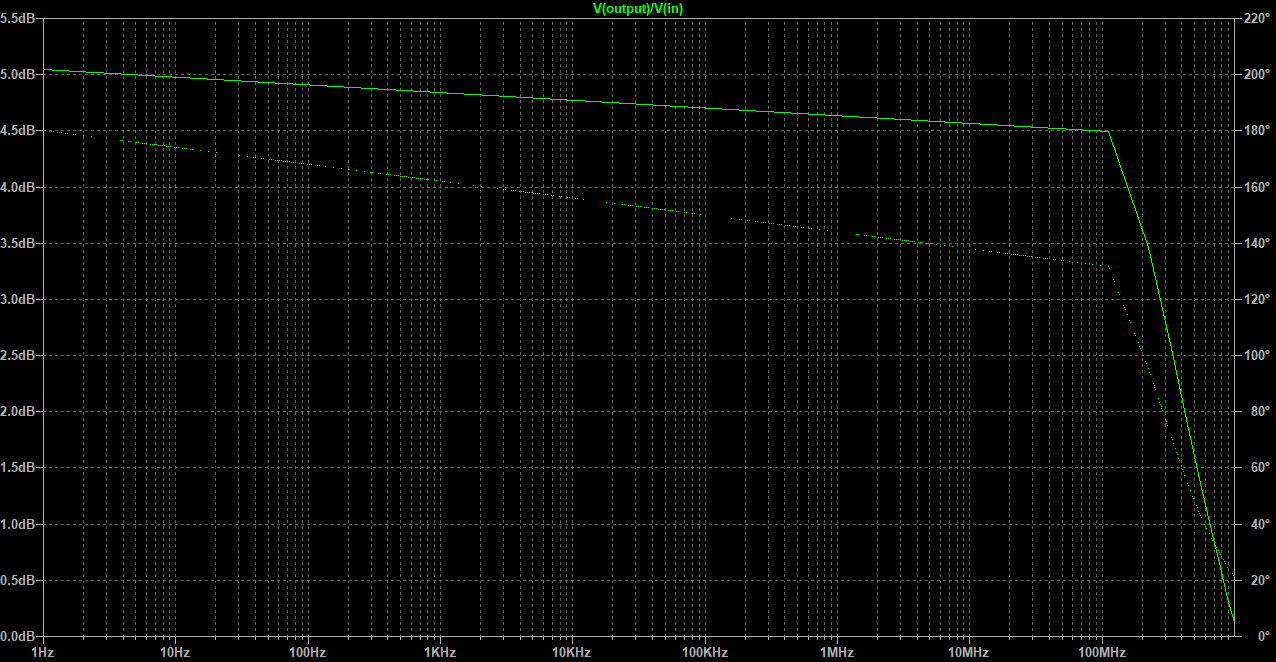
\includegraphics[width=\textwidth]{3_freq_char.png}
    \caption{Частотная характеристика.}
    \label{fig:3_freq_char.png}
\end{figure}

\section*{Выводы}
В данной лабораторной работе был исследован биполярный транзистор. В начале было проведено моделирование работы транзистора в активном режиме с общим эмиттером. Были построены входные и выходные характеристики транзистора, а также некоторые числовые характеристики. Стоит отметить, что значения этих характеристик зависят от схемы включения транзистора. \\
Во второй части была задана рабочая точка транзистора и затем, с помощью отрицательной обратной связи по току была построена схема функционирования (перед этим были рассчитаны параметры резисторов, включенных в схему). \\
В результате, по осциллограммам было определено, что расчеты сделаны верно и транзистор действительно усиливает сигнал до определенных значений. \\
Затем была построена частотная характеристика и можно было убедиться в том, что чем выше частота сигнала, поступающего на вход транзисторного каскада, тем меньше коэффициент усиления по току.

\end{document}